% tex file for time series results
\par \indent For the time being, we considered only a single voxel from the first subject. To specify the orders $p$, $d$, and $q$ for an ARIMA process, we first checked for stationarity by considering the mean function and autocovariance. Visual inspection suggested that the mean function was nonconstant, and additional histograms and quantile-quantile plots suggested a slight skewness with a long right tail. We corrected the skewness using a log transformation, deemed appropriate by the Box-Cox method. The log-transformed data still exhibited a non-constant mean, so we considered using the first difference (i.e. $W_t = Y_t - Y_{t-1}$). The first difference appeared to be much more reasonably stationary. So, we took $d=1$. 

\par Having specified the order for $d$, we turned to the problem of specifying $p$ and $q$. We used a combination of visually inspecting the autocorrelation and partial autocorrelation plots of the first difference, and looking at the Akaike information criteria (AIC) and Bayesian information criteria (BIC) computed from a grid of possible models. The latter method suggested specifying $p=1$ and $q=1$ (based on either the AIC or the BIC), which was also supported by the visual inspections. 

\par We estimated the parameters for an ARIMA(1,1,1) model using the exact maximum likelihood estimator via Kalman filter. The residuals appear to be normally distributed, and its autocorrelation and partial autocorrelation plots also do not raise any red flags. Furthermore, when visually comparing the fitted time series to the true observed data, the ARIMA process seems to approximate the observed data much better than any of the linear regression models. While more work, such as developing more robust methods to assess fit and considering the problem of modeling multiple voxels across multiple subjects, is clearly needed, time series analysis presents a promising direction for further investigation. 

\par In particular, we may be able to forecast future observations based on previous ones. As an example we modeled an ARIMA(1,1,1) process based on the first half of the observations for a single voxel. This process was then used to forecast the second half of the observations. A comparison between the true observations and the forecasted predictions is shown in [Figure \ref{fig:ts-preds}]. While the forecasted observations look reasonable for approximating the true values, more quantitative metrics for assessing performance need to be implemented. 

\begin{figure}[ht]
\centering
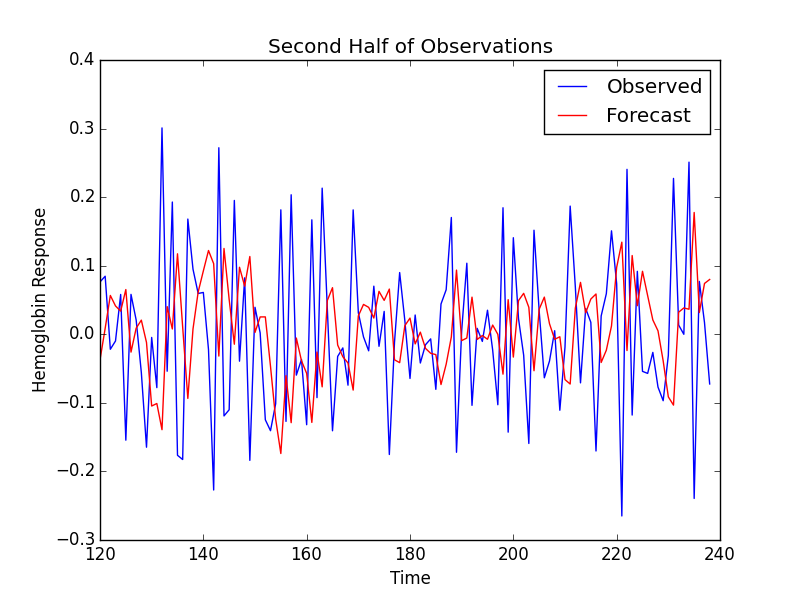
\includegraphics[scale=0.5]{images/ts-preds.png}
\caption{Forecasting the second half of observations based on the first half.}
\label{fig:ts-preds}
\end{figure}

